\documentclass[12pt]{article}
\usepackage{lecture}
\usepackage{graphics}
\usepackage{epstopdf}
\usepackage{html}
\usepackage{url}

\newcommand{\qtl}{{\tt R/qtl}}

\newcommand{\copyrightYears}{2012}

\title{Mapping Quantitative Trait Loci with R/qtl}\index{R/qtl}

\begin{document}

\maketitle

\thispagestyle{first}

\section*{Introduction}

There are two stages to making a QTL map for a particular trait
(once you've scored tens or hundreds of marker loci in tens or
hundreds of $F_2$ or backcross progeny):

\begin{enumerate}

\item Construct a genetic map of your markers.

\item Feed the genetic map, marker data, and phenotype data into QTL
Cartographer and run the analysis.

\end{enumerate}

\noindent Although constructing the genetic map of your markers is
really important step, we're not going to talk about it further. It
is, after all, simply an elaboration of classical Mendelian
genetics.\footnote{Although it gets a {\it lot\/} more complicated
  when you're dealing with tens or hundreds of markers, and you don't
  even know which ones belong on which chromosomes!} 

\section*{The data\footnote{From here on out these notes depend
  heavily on the ``shorter tour of R/qtl'' at
  \url{http://www.rqtl.org/tutorials/}.}}

We're going to focus on the second step. We'll be using data from
Sugiyama et al., {\it Physiological Genomics\/} 10:5�12, 2002 as
distributed from \url{http://www.rqtl.org/sug.csv} As you might have
guessed from the extension on that file, the data is stored in a
standard CSV file. Other formats are possible. They're described in
the documentation, but we'll just deal with CSV files. To see what the
data format looks like, open it up in your favorite spreadsheet
program to take a look.\index{R/qtl!data format}

The data are from an intercross between two lines of inbred mice,
BALB/cj and CBA/CaJ. Its format is fairly straightforward. After the
header rows (lines 1-3), each line provides the data for one
mouse. The first four columns contain phenotypic data: blood pressure,
heart rate, body weight, and heart weight. The next two columns
contain an indicator for the sex of the mouse\footnote{All 1s. Only
  male mice are included in this data set.} and an individual ID. The
remaining columns each correspond to markers (name on row 1, the
chromosome on which they occur on row 2, and the map position on that
chromosome on row 3). The two letters correspond to the alleles
inherited from BALB/cj or CBA/CaJ, B and C
respectively.\footnote{Since the parents were inbred lines, their
  genotypes wer BB and CC.}

Now it's time to get the data into R. To do so, type
\begin{verbatim}
 sug <- read.cross(format="csv", file="sug.csv", genfile="sug.csv",
                   genotypes=c("CC", "CB", "BB"), alleles=c("C", "B"))
\end{verbatim}
This reads data from {\tt sug.csv} and puts it into the R object {\tt
  sug}. Please note that R is case sensitive. If all goes well, you'll
see this on your console after you hit return:
\begin{verbatim}
 --Read the following data:
	 163  individuals
	 93  markers
	 6  phenotypes
 --Cross type: f2 
\end{verbatim}
To get a sense of what's in the data simply type
\begin{verbatim}
 summary(sug)
\end{verbatim}
You should see
\begin{verbatim}
    F2 intercross

    No. individuals:    163 

    No. phenotypes:     6 
    Percent phenotyped: 95.1 95.7 99.4 99.4 100 100 

    No. chromosomes:    19 
        Autosomes:      1 2 3 4 5 6 7 8 9 10 11 12 13 14 15 16 17 18 19 

    Total markers:      93 
    No. markers:        5 7 5 5 5 4 8 4 4 5 6 3 3 5 5 4 4 6 5 
    Percent genotyped:  98.3 
    Genotypes (%):      CC:23.9  CB:50.2  BB:26  not BB:0  not CC:0 
\end{verbatim}
You'll see that more than 95\% of the 163 individuals have been
phenotyped for each of the four traits and that more than 98\% have
been genotyped. You'll also see that all of the loci are
autosomal. You can also {\tt plot(sug)} to get a visual summary of the
data~(Figure~\ref{fig:rqtl-plot-sug}).

\begin{figure}
\begin{center}
\resizebox{\textwidth}{!}{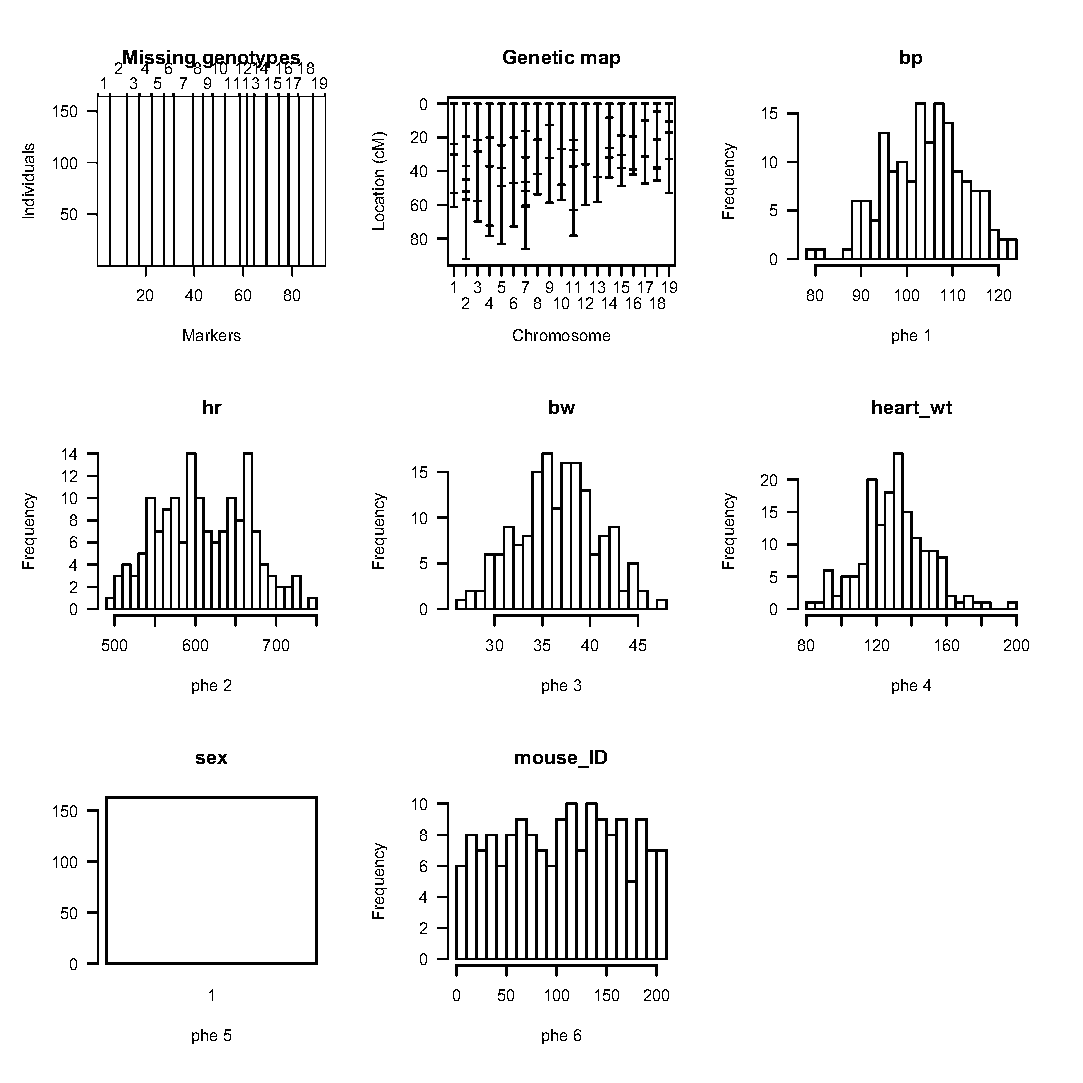
\includegraphics{qtl-rqtl-plot-sug.eps}}
\end{center}
\caption{Results of {\tt plot(sug)}}\label{fig:rqtl-plot-sug}
\end{figure}

The figure in the upper left shows which individuals (rows) are
missing genotype information for particular markers (columns). There's
so little missing genotype data in this data set, it doesn't show
up. The next figure shows the location of markers on the genetic map,
and the remainder summarize the distribution of phenotypes in the data
set.\footnote{The histograms for sex and mouse\_id obviosuly aren't
  very interesting}

\section*{The QTL analysis}\index{R/qtl!QTL analysis}

Now we begin scanning the genome to locate QTLs. First, we have to
calculate the probabilities of the three QTL genotypes in a grid
across the genome. To do that we
\begin{verbatim}
 sug <- calc.genoprob(sug, step=1)
\end{verbatim}
Don't worry when you get nothing back except a command prompt. That's
expected. What you've done is to calculate all of those genotype
probabilities at a grid size of 1cM ({\tt step=1}) across the genome
and stored the results back into {\tt sug}.

Now that we have the QTL genotype probabilities, we can run the QTL
analysis and store the result
\begin{verbatim}
 sug.em <- scanone(sug, pheno.col="bp")
\end{verbatim}
Again, you'll just get the command prompt back.\footnote{Don't worry
  about the warning message. It's expected.}  What you've done is to
store the results in an object called {\tt sug.em}.\footnote{I called
  it {\tt sug.em} because {\tt scanone()} is using the EM algorithm to
  obtain maximum-likelihood estimates of the parameters. Other
  algorithms are available, but we won't discuss them.} This analysis
will locate only QTLs that influence blood pressure ({\tt
  pheno.col=''bp''}). If I'd wanted to analyze one of the other
traits, I would have specified {\tt pheno.col=''hr''}, {\tt
  pheno.col=''bw''}, or {\tt pheno.col=''heart\_wt''}. If I summarize
the results to this point ({\tt summary(sug.em)}, I'll get a report of
the maximum LOD score on each chromosome.
\begin{verbatim}
          chr   pos   lod
D1MIT36     1 76.73 1.449
c2.loc77    2 82.80 1.901
c3.loc42    3 52.82 1.393
c4.loc43    4 47.23 0.795
D5MIT223    5 86.57 1.312
c6.loc26    6 27.81 0.638
c7.loc45    7 47.71 6.109
c8.loc34    8 54.90 1.598
D9MIT71     9 27.07 0.769
c10.loc51  10 60.75 0.959
c11.loc34  11 38.70 2.157
D12MIT145  12  2.23 1.472
c13.loc20  13 27.26 1.119
D14MIT138  14 12.52 1.119
c15.loc8   15 11.96 5.257
c16.loc31  16 45.69 0.647
D17MIT16   17 17.98 1.241
D18MIT22   18 13.41 1.739
D19MIT71   19 56.28 0.402
\end{verbatim}

To determine whether any of the markers are associated with the blood
pressure phenotype more strongly than we would expect at random, we
perform a permutation test.\index{R/qtl!permutation test}
\begin{verbatim}
 sug.perm <- scanone(sug, pheno.col="bp", n.perm=5000)
\end{verbatim}
You'll get a progress report as the permutations proceed, but be
prepared to wait quite awhile. Each individual permutation reruns the
entire {\tt scanone()} analysis with phenotypes and genotypes
randomized relative to one another. This gives us a distribution of
LOD scores expected at random, and we'll use this to set a threshold
that takes account of the multiple comparisons we make when we do
separate likelihood-ratio tests at every potential QTL position in the
genome.

With the permutations in hand, we can now summarize the results of the
analysis and identify the position of QTLs for blood pressure (to a
1cM resolution).\index{R/qtl!identifying QTLs}
\begin{verbatim}
  summary(sug.em, perms=sug.perm, alpha=0.05, p.values=TRUE)
\end{verbatim}
By specifying {\tt alpha=0.05}, all peaks with a genome-adjusted
p-value of less than 0.05 will be included in the summary. By
specifying {\tt p.values=TRUE} we ensure that only columns with
genome-adjusted p-values are considered.\footnote{Since we included
  all markers in our permutation test, this will simply include all
  columns.} The summary is very short and simple:
\begin{verbatim}
         chr  pos  lod
c7.loc45   7 47.7 6.11
c15.loc8  15 12.0 5.26
\end{verbatim}
It tells us that only two QTLs have a significant association with
blood pressure, one on chromosome 7 at 47.7cM, the otehr on chromosome
15 at 12.0cM.

Finally, we visualize the effects of the QTLs on chromosome 7 and
chromosome 15.\index{R/qtl!visualizing QTL effects}
\begin{verbatim}
  sug <- sim.geno(sug)
  effectplot(sug, pheno.col="bp", mname1="7@47.7")
  effectplot(sug, pheno.col="bp", mname2="15@12")
  effectplot(sug, pheno.col="bp", mname1="7@47.7", mname2="15@12")
  effectplot(sug, pheno.col="bp", mname1="15@12", mname2="7@47.7")
\end{verbatim}
You'll see the results in Figure~\ref{fig:qtl-rqtl-effects}. The top
two figures show the phenotypic means associated with markers on
chromosome 7 and 15 respectively. The bottom two figures show how the
phenotype depends on the genotype at both QTLs. The QTL on chromosome
15 (figure on the right) seems to have almost purely additive
effects. The heterozygote is very close to intermediate between the
two homozygotes. The QTL on chromosome 7, however, has substantial
non-additive effects. Blood pressure of heterozygotes appears to be
lower than that of either homozygote. The interaction plots suggests
epistatic interactions between the loci. The lines aren't parallel. 

\begin{figure}
\resizebox{\textwidth}{!}{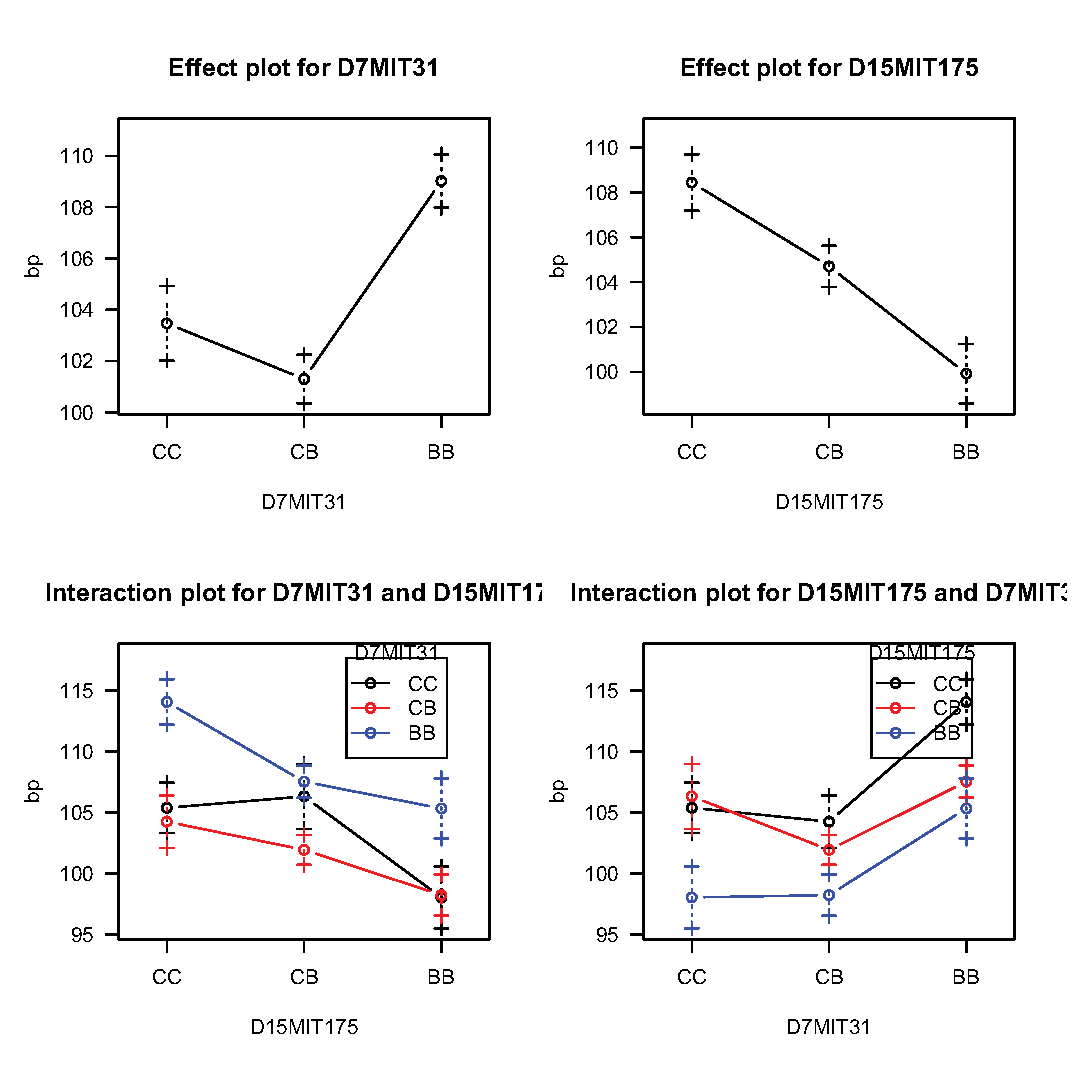
\includegraphics{qtl-rqtl-effects.eps}}
\caption{Effect plots for the QTLs on chromosome 7 and chromosome
  15}\label{fig:qtl-rqtl-effects} 
\end{figure}

We can get numerical estimates of the means and standard errors by
changing those statements just a little.\index{R/qtl!estimating QTL
  effects} 
\begin{verbatim}
  print(effectplot(sug, pheno.col="bp", mname1="7@47.7", draw=FALSE))
$Means
D7MIT31.CC D7MIT31.CB D7MIT31.BB 
  103.4679   101.3002   109.0165 

$SEs
D7MIT31.CC D7MIT31.CB D7MIT31.BB 
 1.4486284  0.9499457  1.0415715 

  print(effectplot(sug, pheno.col="bp", mname2="15@12", draw=FALSE))
$Means
D15MIT175.CC D15MIT175.CB D15MIT175.BB 
   108.43902    104.70130     99.91892 

$SEs
D15MIT175.CC D15MIT175.CB D15MIT175.BB 
    1.258112     0.918049     1.324373 
\end{verbatim}

We estimate additive and dominance effects associated with each marker
from a linear regression
\[
y_i = \beta_0 + \alpha_ia + \delta_id
\]
where $\alpha_i = (-1,0,1)$ and $\delta_i = (0, 1, 0)$ for genotypes
CC, CB, and BB, respectively. With $a$ and $d$ estimated in this way
we can specify the genotypic values as

\begin{center}
\begin{tabular}{ccc}
\hline\hline
CC & CB & BB \\
\hline
$\bar x - a$  & $\bar x + d$  & $\bar x + a$ \\
\hline
\end{tabular}
\end{center}

\noindent Doing that regression may sound hard, but it's actually quite
easy.
\begin{verbatim}
  print(effectscan(sug, pheno.col="bp", draw=FALSE))
\end{verbatim}
You'll get a very long table as a result. Here I just pull out the
lines corresponding to the two QTLs we identified.
\begin{verbatim}
          chr   pos           a            d
D7MIT31     7 49.01  2.77491094 -4.950729964
D15MIT175  15  3.96 -4.26005274  0.522327047
\end{verbatim}

\ccLicense{}

\end{document}
